 \section{Entropy and Mutual Information}
\label{sec:Entropy and Mutual Information}
\begin{rem}
  Neural encoding and decoding focus on the question ``What does the response
of a neuron tell us about a stimulus?'' In this chapter we consider
a related but different question ``How much does the neural response tell
us about a stimulus?'' The techniques of information theory allow us to
answer this question in a quantitative manner. Furthermore, we can use
them to ask what forms of neural response are optimal for conveying information
about natural stimuli.
\end{rem}

\begin{defn}
   \emph{Information theory} is a general framework for quantifying the ability of a coding scheme or a communication channel (such as the optic nerve) to convey information.
\end{defn}

\begin{asm}
In information theory, it is assumed that the code involves a number of symbols, and that the coding and transmission processes are stochastic and noisy.
\end{asm}

\begin{defn}
  \label{def:entropy}
  \emph{Entropy} is a measure of the theoretical capacity of a code to convey information.
\end{defn}

\begin{defn}
  \label{def:mutualInformation}
  \emph{Mutual information} is a measure of how much of that capacity is actually used when the code is employed to describe a particular set of data.
\end{defn}

\begin{rem}
  Communication channels, if they are noisy, have only limited capacities to convey information. The techniques of information theory are used to evaluate these limits and find coding schemes that saturate them.
\end{rem}

\begin{ntn}
  In neuroscience applications, the symbols we consider are neuronal responses, and the data sets they describe are stimulus characteristics. We discuss cases in which the symbols consist of responses described by spike-count firing rates $r$ as the simplified descriptions of the response of a neuron that reduce the number of possible ``symbols'' (i.e., responses) that need to be considered. %We also consider the extension to continuous-valued firing rates.
  In the following, we just consider neuroscience applications.
\end{ntn}

\begin{rem}
  Because a reduced description of a spike train can carry no more information than the full spike train itself, this approach provides a lower bound on the actual information carried by the spike train.
\end{rem}


\subsection{Entropy}
\label{sec:entropy}

\begin{fac}
  Entropy is a quantity that, roughly speaking, measures how ``interesting'' or ``surprising'' a set of responses is.
\end{fac}

\begin{exm}
  The most widely used measure of entropy, due to Shannon, expresses the ``surprise'' associated with seeing a response rate $r$ as a function of the probability of getting that response, $h(P[r])$, and quantifies the
  entropy as the average of $h(P[r])$ over all possible responses. The function
  $h(P[r])$, which acts as a measure of surprise, is chosen to satisfy a number of conditions:
  \begin{enumerate}[(1)]
  \item  $h(P[r])$ should be a decreasing function of $P[r]$
    because low probability responses are more surprising than high probability responses.
  \item The surprise measure for a response that consists of two independent spike counts should be the sum of the measures for each spike count separately. Suppose we record rates $r_1$ and $r_2$ from two neurons that respond independently of each other, the additivity condition requires that
    \begin{equation}
      \label{equ:4.1}
      h(P[r_1]P[r_2])=h(P[r_1])+h(P[r_2]).
    \end{equation}
  \end{enumerate}
  The logarithm is the only function that satisfies such an identity for all $P$.
  Thus, it only remains to decide what base to use for the logarithm. By convention, base 2 logarithms are used so that information can be compared easily with results for binary systems. Information is reported in units of ``bits'', with
  \begin{equation}
    \label{equ:4.2}
    h(P[r])=-\log_2P[r],
  \end{equation}
  where the minus sign makes $h$ a decreasing function of its argument as required.
\end{exm}

\begin{rem}
  Note that information is really a dimensionless number. The bit, like the radian for angles, is not a dimensional unit but a reminder that a particular system is being used.
\end{rem}

\begin{defn}
  \label{def:ShannonEntropy}
  Equation \ref{equ:4.2} quantifies the surprise or unpredictability associated with a particular response. \emph{Shannon's entropy} is this measure averaged entropy over all responses,
\begin{equation}
  \label{equ:4.3}
  H=-\sum\limits_rP[r]\log_2P[r],
\end{equation}
where $r$ is spike-count firing rates (i.e., the number of spikes divided by the trial duration).
\end{defn}

\begin{ntn}
  In the following, the entropy means Shannon's entropy.
\end{ntn}

\begin{exm}
   The neuron responds in only two possible ways, either with rate $r_+$ or $r_-$. In
this case, there are only two nonzero terms in Equation \ref{equ:4.3}, and, using
the fact that $P[r_-]=1-P[r_+]$, the entropy is
\begin{equation*}
  \label{equ:4.4}
  H=-(1-P[r_+])\log_2(1-P[r_+])-P[r_+]\log_2(P[r_+]).
\end{equation*}
This entropy, plotted in figure, takes its maximum value of 1 bit when
$P[r_-]=P[r_+]=1/2$. Thus, a code consisting of two equally likely responses has one bit of entropy.
\begin{center}
    \label{fig:4-1}
  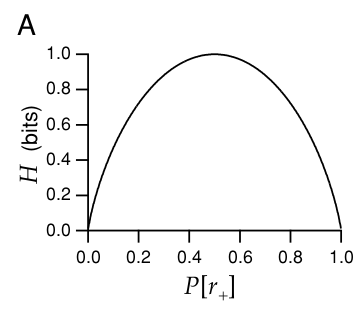
\includegraphics[scale = 0.4]{./png/4-1A}
\end{center}
\end{exm}

\subsection{Mutual Information}
\begin{rem}
  Entropy is a measure of response variability, but it does not tell us anything about the source of that variability. A neuron can provide information about a stimulus only if its response variability is correlated with changes in that stimulus, rather than being purely random or correlated with other unrelated factors. Mutual information is an entropy-based measure related to this idea.
\end{rem}

\begin{thm}
  \label{thm:entropy of the responses to a given stimulus}
  The entropy of the responses to a given stimulus $s$ is
  \begin{equation}
    \label{equ:4.5}
    H_s=-\sum\limits_rP[r|s]\log_2P[r|s].
  \end{equation}
\end{thm}
\begin{proof}
  The entropy of the responses evoked by repeated presentations of a given stimulus $s$ is computed using the conditional probability $P[r|s]$, the probability of a response at rate $r$ given that stimulus $s$. This proof is completed by Definition \ref{def:ShannonEntropy}.
\end{proof}

\begin{defn}
  \label{defn:noise entropy}
  The \emph{noise entropy} is the entropy associated with that part of the response variability that is not due to changes in the stimulus, but arises from other sources. It can be obtained by averaging the quantity \ref{equ:4.5} over all the stimuli,
  \begin{equation}
    \begin{aligned}
      \label{equ:4.6}
      H_{\text{noise}}&=\sum_s{P[s]H_s}\\
      &=-\sum\limits_{s,r}{P[s]P[r|s]\log_2{P[r|s]}}.
    \end{aligned}
  \end{equation}
\end{defn}

\begin{defn}
  \label{defn:mutual-information}
  The \emph{mutual information} is the difference between the total response entropy and the noise entropy, which from equations \ref{equ:4.3} and \ref{equ:4.6} gives
  \begin{equation}
    \begin{aligned}
      \label{equ:4.7}
      I_{\text{m}}&=H-H_{\text{noise}}\\
      &=-\sum\limits_{r}{P[r]\log_2P[r]+\sum\limits_{s,r}P[s]P[r|s]\log_2P[r|s]}.
    \end{aligned}
  \end{equation}
\end{defn}

\begin{prop}
  The mutul information defined in Equation \ref{equ:4.7} can be written in two forms as follows,
  
  \begin{align}
    \label{equ:4.9}   I_{\text{m}}&=\sum\limits_{s,r}{P[s]P[r|s]\log_2\left(
                                   \frac{P[r|s]}{P[r]} \right)},\\
    \label{equ:4.11}  I_{\text{m}}&=\sum\limits_{s,r}{P[r,s]\log_2\left( \frac{P[r,s]}{P[r]P[s]} \right)}.
  \end{align}
  \begin{proof}
    The first equation can be derived by using 
    \begin{equation}
      \label{equ:4.8}
      P[r]=\sum\limits_s{P[s]P[r|s]},
    \end{equation}
    and writing the difference of the two logarithms in Equation \ref{equ:4.7} as the logarithm of the ratio of their arguments.
    Recall from chapter 3 that
    \begin{equation}
      \label{equ:4.10}
      P[r,s]=P[s]P[r|s]=P[r]P[s|r],
    \end{equation}
    where $P[r,s]$ is the joint probability of stimulus $s$ appearing and response $r$ being evoked. This equation can be used to derive the second form of the above equations for the mutual information.
  \end{proof}
\end{prop}

\begin{rem}
  Equation \ref{equ:4.11} reveals that the mutual information is symmetric with respect to interchange of $s$ and $r$, which means that the mutual information that a set of responses conveys about a set of stimuli is identical to the mutual information that the set of stimuli conveys about the responses.
\end{rem}


\begin{thm}
  The mutul information also satisfies
  \begin{equation}
    \label{equ:4.12}
    I_{\text{m}}=-\sum\limits_{s}{P[s]\log_2P[s]}+\sum\limits_{s,r}{P[r]P[s|r]\log_2P[s|r]},
  \end{equation}
  which is the same as Equation \ref{equ:4.7}, except that the roles of the stimulus and the response have been interchanged.
  \begin{proof}
    Applying the second equality of Equation \ref{equ:4.10} in Equation \ref{equ:4.11} completes this proof.
  \end{proof}
\end{thm}

\begin{rem}
  Equation \ref{equ:4.12} shows how response variability limits the ability of a spike train to carry information. The second term on the right side, which is negative, is the average uncertainty about the identity of the stimulus given the response, and reduces the total stimulus entropy represented by the first term.
\end{rem}

\begin{exm}
  Suppose that the responses of the neuron are completely unaffected by the identity of the stimulus. In this case, $P[r|s] = P[r]$, and from Equation \ref{equ:4.9} it follows immediately that $I_{\text{m}} = 0$.
\end{exm}

\begin{exm}
  Suppose that each stimulus $s$ produces a unique and distinct response $r_s$. Then, $P[r_s]= P[s]$ and $P[r|s]$ is 1 if $r=r_s$ and 0 otherwise. This causes the sum over $r$ in Equation \ref{equ:4.9} to collapse to just one term, and the mutual information becomes
  \begin{equation}
    \label{equ:4.13}
    I_{\text{m}}=\sum\limits_sP[s]\log_2\left( \frac{1}{P[r_s]} \right)=-\sum\limits_{s}{P[s]\log_2P[s]},
  \end{equation}
  where the last equality, which follows from the fact that $P[r_s] = P[s]$, is the entropy of the stimulus. Thus, with no variability and a one-to-one map from stimulus to response, the mutual information is equal to the full stimulus entropy.
\end{exm}
\begin{exm}
  Imagine that there are only two possible stimulus values, which we label $+$ and $-$, and that the neuron responds with just two rates, $r_+$ and $r_-$. We associate the response $r_+$ with the + stimulus, and the response $r_-$ with the $-$ stimulus, but the encoding is not perfect. The probability of an incorrect response is $P_X$, meaning that for the correct responses $P[r_+|+]=P[r_-|-]=1-P_X$, and for the incorrect responses $P[r_+|-]=P[r_-|+]=P_X$. We assume that the two stimuli are presented with equal probability so that $P[r_+]=P[r_-]=1/2$, which makes the full response entropy 1 bit. The noise entropy is $-(1-P_{X})\log_2(1-P_X)-P_X\log_2 P_X$. Thus, the mutual information is
  \begin{equation}
    \label{equ:4.14}
    I_{\text{m}}=1+(1-P_X)\log_2(1 - P_X) + P_X\log_{2} P_X,
  \end{equation}
  which is plotted in the following figure. When the encoding is error-free ($P_X=0$),
  the mutual information is 1 bit, which is equal to both the full response
  entropy and the stimulus entropy. When the encoding is random ($P_X = 1/2$), the mutual information goes to 0.
  \begin{center}
    \label{fig:4-1B}
    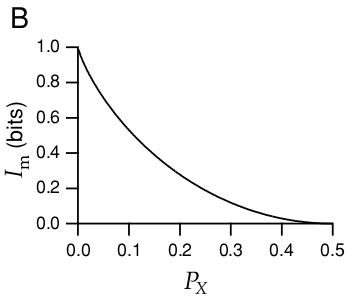
\includegraphics[scale = 0.4]{./png/4-1B}
  \end{center}
\end{exm}

\begin{rem}
  It is instructive to consider this example from the perspective of decoding. We can think of the neuron as being a communication channel that reports noisily on the stimulus. From this perspective, we want to know the probability that a $+$ was presented, given that the response $r_+$ was recorded. By Bayes theorem, this is $P[+|r_+] = P[r_+|+]P[+]/P[r_+] = 1 - P_X$. Before the response is recorded, the expectation was that $+$ and $-$ were equally likely. If the response $r_+$ is recorded, this expectation changes to $1 - P_X$. The mutual information measures the corresponding reduction in uncertainty or, equivalently, the tightening of the posterior distribution due to the response.
\end{rem}

\begin{rem}
  The mutual information is related to a measure used in statistics called the Kullback-Leibler (KL) divergence.
\end{rem}

\begin{defn}
  \label{defn:Kullback-Leibler (KL) divergence}
  The \emph{Kullback-Leibler(KL) divergence} between one probability distribution $P[r]$ and another distribution $Q[r]$ is
  \begin{equation}
    \label{equ:4.15}
    D_{\text{KL}}(P,Q)=\sum\limits_{r}P[r]\log_2\left( \frac{P[r]}{Q[r]} \right).
  \end{equation}
\end{defn}
\begin{thm}
  \label{thm:KLnon-negative}
  The KL divergence has a property normally associated with a distance measure, $D_{\text{KL}}(P, Q) \geq 0$ with equality if and only if $P=Q$.
  \begin{proof}
    The logarithm is a concave function, which means that $\log_2\left< z \right>\geq \left<\log_2z  \right>$
    where the angle brackets denote averaging with respect to some probability distribution and $z$ is any positive quantity. The equality holds only if $z$ is a constant. If we consider this relation, known as Jensen's inequality, with $z = P[r]/Q[r]$ and the average defined over the probability distribution $P[r]$, we find   
    \begin{equation}
      \begin{aligned}
        \label{equ:4.56}
        -D_{\text{KL}}(P,Q)&=\sum\limits_{r}{P[r]\log_2\left(
            \frac{Q[r]}{P[r]}  \right)}\\
        &\leq \log_2\left( \sum\limits_r{P[r] \frac{Q[r]}{P[r]}} \right)=0.
      \end{aligned}
    \end{equation}
    The last equality holds because $Q[r]$ is a probability distribution and thus
    satisfies $\sum_{r}Q[r]=1$. Equation \ref{equ:4.56} implies that $D_{\text{KL}}(P,Q)\geq 0$, with
    equality holding if and only if $P[r]=Q[r]$.
  \end{proof}   
\end{thm}

\begin{coro}
  A similar result holds for the
  Kullback-Leibler divergence between two probability densities,
  \begin{equation}
    \label{equ:4.57}
    D_{\text{KL}}(p,q)=\int {p[r]\log_2\frac{p[r]}{q[r]}}dr\geq 0.
  \end{equation}
\end{coro}

\begin{thm}
  \label{thm:MutualKL}
  The mutual information is the KL divergence between the distributions $P[r,s]$ and $P[r]P[s]$.
\end{thm}
\begin{proof}
  This is directly from Definition \ref{defn:Kullback-Leibler (KL) divergence} and Equation \ref{equ:4.11}.
\end{proof}

\begin{rem}
  If the stimulus and the response were independent of one another, $P[r,s]$ would be equal to  $P[r]P[s]$. Thus, the mutual information is the KL divergence between the actual probability distribution $P[r,s]$ and the value it would take if the stimulus and response were independent.
\end{rem}

\begin{coro}
  The mutual information cannot be negative. In addition, it can never be larger than either the full response entropy or the entropy of the stimulus set.
\end{coro}
\begin{proof}
  The first conclusion is directly from theorems \ref{thm:MutualKL} and \ref{thm:KLnon-negative}. The second is from equations \ref{equ:4.7} and \ref{equ:4.12}.
\end{proof}

\subsection{Entropy and Mutual Information for Continuous Variables}

\begin{rem}
  Up to now we have characterized neural responses using discrete spike count rates. As in chapter 3, it is often convenient to treat these rates instead as continuous variables. %If we could measure the value of a continuously defined firing rate with unlimited accuracy, it would be possible to convey an infinite amount of information using the endless sequence of decimal digits of this single variable. Of course, practical considerations always limit the accuracy with which a firing rate can be measured or conveyed.
\end{rem}

\begin{fac}
  If we could measure the value of a continuously defined firing rate with unlimited accuracy, it would be possible to convey an infinite amount of information using the endless sequence of decimal digits of this single variable. Of course, practical considerations always limit the accuracy with which a firing rate can be measured or conveyed.
\end{fac}

\begin{rem}
  To define the entropy associated with a continuous measure of a neural response, we must include some limit on the measurement accuracy.
%   The effects of this limit typically cancel in computations of mutual information because the mutual information is the difference between two entropies.
\end{rem}


\begin{prop}
  For a continuously defined firing rate, the entropy with measurement accuracy $\Delta r$ satisfies
  \begin{equation}
    \label{equ:4.16}
    \begin{aligned}
      H = -\sum{p[r]\Delta r\log_2p[r]}-\log_2\Delta r.  
    \end{aligned}
  \end{equation}
  \begin{proof}
    For a continuously defined firing rate, the probability of the firing rate lying in the range between $r$ and $r+\Delta r$, for small $\Delta r$, is expressed in terms of a probability density as $p[r]\Delta r$. Summing over discrete bins of size $\Delta r$, we find, by analogy with equation \ref{equ:4.3},
    \begin{displaymath}
      \begin{aligned}
        H&= -\sum{p[r]\Delta r\log_2(p[r]\Delta r)}\\
        &= -\sum{p[r]\Delta r\log_2p[r]}-\log_2\Delta r,
      \end{aligned}
    \end{displaymath}
    where the last equality follows from the fact that the sum of the response probabilities is 1.
  \end{proof}
\end{prop}

\begin{rem}
  We would now like to take the limit $\Delta r \rightarrow 0$ but we
cannot, because the $\log_2\Delta r$ term diverges in this limit. This divergence reflects the fact that a continuous variable measured with perfect accuracy has infinite entropy.
\end{rem}



\begin{thm}
  In the limit $\Delta r\to 0$ with the sum replaced by an integral, we can write
  \begin{equation}
    \label{equ:4.17}
    \lim\limits_{\Delta r\to 0}\{H+\log_2\Delta r\}=-\int{p[r]\log_2p[r]dr},
  \end{equation}
  where $\Delta r$ is best thought of as a limit on the resolution with which the firing rate can be measured.
\end{thm}

\begin{rem}
  If two entropies computed with the same resolution are subtracted,
  the troublesome term involving $\Delta r$ cancels, and we can
  proceed without knowing its precise value.
\end{rem}

\begin{defn}
  The integral on the right side of Equation \ref{equ:4.17} is sometimes called the \emph{differential entropy}.
\end{defn}


\begin{prop}
  The noise entropy, for a continuous variable like the firing rate, can be written in a manner similar to the response entropy Equation \ref{equ:4.17}, except that the conditional probability density $p[r|s]$ is used:
\begin{equation}
  \label{equ:4.18}
  \lim\limits_{\Delta r\rightarrow 0}\{H_{\text{noise}}+\log_2\Delta
    r\}=-\iint{p[s]p[r|s]\log_2p[r|s]drds}.
\end{equation}
\end{prop}

\begin{prop}
  The mutual information is the difference between the expressions in equations
  \ref{equ:4.17}  and \ref{equ:4.18},
  \begin{equation}
    \label{equ:4.19}
    I_{\text{m}}=\iint{p[s]p[r|s]\log_{2}\left( \frac{p[r|s]}{p[r]} \right)drds}.
  \end{equation}
  \begin{proof}
    Here the factor of $\log_2\Delta r$ cancels  because both entropies are evaluated at the same resolution.
  \end{proof}
\end{prop}

\begin{rem}
  There are some differences and relationships%for the measure of how tightly the responses determine the stimulus
  between Fisher information and mutual information:
  \begin{enumerate}[(i)]
  \item  We described the Fisher information as a local measure of
how tightly the responses determine the stimulus. The Fisher information is local because it depends on the expected curvature of the likelihood
$P[\mathbf{r}|s]$ (typically for the responses of many cells) evaluated
at the true stimulus value.
\item The mutual information is a global measure in the sense that
it depends on the average overall uncertainty in the decoding distribution
$p[s|\mathbf{r}]$, including values of $s$ both close to and far from
the true stimulu $s$.
If the decoding distribution $p[s|\mathbf{r}]$ has a single peak about the true stimulus, the Fisher information and the mutual information are closely
related.
??????????????????????????????????????????
\end{enumerate}
\end{rem}





 %%%Local Variables:
%%% mode: latex
%%% TeX-master: "../notesOnFluidMechanics"
%%% End:
